% note.tex — φ^3+φ^4 理論：模型の定義と1ループの構造（d = 4）
% コンパイル: lualatex note.tex（目次と参照の解決のため2〜3回）
\documentclass[a4paper,10pt]{ltjsarticle}
\usepackage[margin=20mm]{geometry}
\usepackage[haranoaji,deluxe]{luatexja-preset}
\ltjsetparameter{jacharrange={-3}}
\usepackage{amsmath,amssymb}
\usepackage{booktabs,tabularx,array}
\usepackage[table]{xcolor}
\usepackage{tikz}
\usetikzlibrary{arrows.meta,calc,positioning}
\usepackage[font=small,labelfont=bf]{caption}
\usepackage{graphicx}
\usepackage{xurl}
\usepackage{hyperref}
\hypersetup{colorlinks=true,linkcolor=blue!50!black,citecolor=green!40!black,urlcolor=blue!60!black,
  pdftitle={phi^3+phi^4 theory: model and one-loop structure},pdfauthor={}}

\renewcommand{\jsParagraphMark}{\textcolor{black!65}{\rule[-0.02\zw]{0.62\zw}{0.62\zw}}\hspace{0.35\zw}}
\newcommand{\dd}{\mathrm{d}}

\tikzset{
  prop/.style={thick},
  vtx/.style={circle,fill=black,inner sep=1.3pt},
  ctv/.style={circle,draw=black,fill=white,inner sep=0pt,minimum size=7pt,path picture={
      \draw (path picture bounding box.north west) -- (path picture bounding box.south east)
            (path picture bounding box.south west) -- (path picture bounding box.north east);}},
  mom/.style={-{Stealth[length=1.6mm]},thin},
  lab/.style={font=\small,align=center},
}

\title{$\phi^3+\phi^4$ 理論：模型の定義と1ループの構造（$d=4$）}
\author{}
\date{2026年10月10日}

\begin{document}
\maketitle

\begin{abstract}
$\phi^3$ 理論のノート~\cite{phi3note} に続き、4点の自己相互作用を加えた実スカラー1つの $\phi^3+\phi^4$ 理論を $d=4$ で調べる。目的は二つである。一つは、結合が二つになったときの1ループの繰り込みの構造を手で求め、$\phi^3$ 理論と同じ手順でツールと突き合わせることである。もう一つは、この模型の物理、とくに真空の構造と偽の真空の崩壊を調べることである。手計算では、Feynman 則と対称性因子、1ループの1PI 関数、$\overline{\mathrm{MS}}$ の対抗項 $\delta_m=(g^2+\lambda m^2)\Delta_{\mathrm{UV}}/(2(4\pi)^2)$、$\delta_g=3g\lambda\Delta_{\mathrm{UV}}/(2(4\pi)^2)$、$\delta_\lambda=3\lambda^2\Delta_{\mathrm{UV}}/(2(4\pi)^2)$ を求めた。繰り込み群は $\beta_\lambda=3\lambda^2/(4\pi)^2$、$\beta_g=3g\lambda/(4\pi)^2$、$\mu\,\dd m^2/\dd\mu=(g^2+\lambda m^2)/(4\pi)^2$ で、有効ポテンシャルからも同じものが得られる。真空の構造は一つの数 $\alpha=3\lambda m^2/g^2$ で決まり、$\alpha<1$ では $\phi=0$ が偽の真空になる。ヒッグスの自己結合に読み替えると $\alpha=\kappa_4/\kappa_3^2$ で、標準模型はちょうど $\alpha=1$（縮退した二つの極小）にあたる。検算の手順 (1) として、FeynRules の模型ファイルから FeynArts 模型と UFO を書き出し、Feynman 則と MadGraph の図の数を確かめた。手順 (2) では、木の振幅が FeynCalc の結果と記号として一致し、MadGraph の断面積が数値積分と統計誤差の範囲で一致した。手順 (3) では、1PI 関数の図、極、対抗項が記号として一致し、有限部分が Package-X・LoopTools・COLLIER の間で相対 $10^{-11}$ 以内で一致した。手順 (4) では、1ループの $\phi\phi\to\phi\phi$ 振幅（42図）が FeynCalc と FormCalc の両方で手計算と記号として一致し、四つの経路の数値が相対 $4\times10^{-12}$ 以内で一致し、虚部がユニタリー性を満たした。導出はすべて付録に省略なく載せる。
\end{abstract}

\tableofcontents

\section{目的と問い}\label{sec:intro}

本ノートの問いは二つである。\textbf{第一に、$\phi^3$ 理論に4点の自己相互作用 $\lambda\phi^4/4!$ を加えると、$d=4$ の1ループの紫外発散と繰り込みの構造はどう変わるか。そして、その構造を $\phi^3$ 理論と同じ手順でツールと突き合わせられるか。第二に、この模型の物理について何が言えるか。}とくに、摂動論が使える結合の範囲と、真空の構造、偽の真空の崩壊を調べる。

第一の問いを立てる理由は、$\phi^3$ 理論~\cite{phi3note} では $d=4$ の繰り込みが質量の対抗項だけで済み、$d=4$ で結合定数の繰り込みと $\beta$ 関数をツールで確かめる機会がなかったからである。$\lambda\phi^4$ を加えると、$d=4$ でも結合の対抗項 $\delta_g$、$\delta_\lambda$ が現れ、$\beta$ 関数が0でなくなる。1PI の4点関数には、2点積分（$\lambda^2$）、3点積分（$\lambda g^2$）、4点積分（$g^4$）が同時に現れる。第二の問いを立てる理由は、一つの実スカラーの $\phi^3+\phi^4$ のポテンシャルが、ユニタリーゲージで書いた標準模型（SM）のヒッグスのポテンシャルの、3点と4点の結合を独立に変えたものと同じ形をしているからである。$\phi^3$ 理論で作った部分波と bounce の道具を、そのまま意味のある問題に使える。

求める量は五つである。(i) Feynman 則と対称性因子。(ii) 1ループの1PI 関数（1点〜4点）の紫外発散部分と、$\overline{\mathrm{MS}}$ の対抗項。(iii) 繰り込まれた1PI 関数と、繰り込み群の係数（$\beta_\lambda$、$\beta_g$、質量の走り）。(iv) $\phi\phi\to\phi\phi$ の木の振幅と1ループの振幅、およびその S 行列要素。(v) 応用として、部分波のユニタリー性の限界、真空の構造、偽の真空の崩壊率（bounce の作用は $d=4$ と $d=3$、前因子は $d=4$）。手計算とツールの間で求める一致は、$\phi^3$ 理論と同じく、発散部分と対抗項では記号として完全な一致、有限部分では数値基準点での倍精度の一致である。

本ノートの構成は次の通りである。第~\ref{sec:setup} 節で模型と前提を定める。第~\ref{sec:results} 節で上の (i)〜(iv) の手計算の結果と、(v) の前提になる真空の構造を述べる。第~\ref{sec:plan} 節で、これらを各ツールと突き合わせる計画を定める。第~\ref{sec:checks} 節で、その結果を示す（現在は手順 (4) まで）。第~\ref{sec:discussion} 節で未決の点と今後の手順をまとめる。導出は\ref{app:rules}〜\ref{app:vacuum} にある。

\section{設定}\label{sec:setup}

模型は、質量 $m$ を持つ実スカラー場 $\phi$ が1つだけあり、3次と4次の自己相互作用を持つ理論である。ラグランジアン密度は
\begin{equation}
\begin{aligned}
\mathcal{L}={}&\frac12\,\partial_\mu\phi\,\partial^\mu\phi-\frac12 m^2\phi^2-\frac{g\mu^{\epsilon}}{3!}\,\phi^3-\frac{\lambda\mu^{2\epsilon}}{4!}\,\phi^4+Y\phi\\
&+\frac12\,\delta_Z\,\partial_\mu\phi\,\partial^\mu\phi-\frac12\,\delta_m\phi^2-\frac{\delta_g\mu^{\epsilon}}{3!}\,\phi^3-\frac{\delta_\lambda\mu^{2\epsilon}}{4!}\,\phi^4
\end{aligned}
\label{eq:L}
\end{equation}
とする。1行目が繰り込まれた量で書いた模型、2行目が対抗項である。$\lambda=0$ とすると $\phi^3$ 理論のノート~\cite{phi3note} のラグランジアンになる。線形項 $Y\phi$ は、ループが作る1点関数（タドポール）を各次数でちょうど打ち消し、$\langle\phi\rangle=0$ を保つために置く。

\paragraph{前提。}本ノートは次の前提に立つ。
\begin{enumerate}
\item 計量は $(+,-,-,-)$、$\hbar=c=1$ とする。
\item 場は質量 $m$ の実スカラー1つで、相互作用は $\phi^3$ と $\phi^4$ だけとする。$\lambda\ge0$ とし、ポテンシャルは下に有界である。$m^2>0$ なので、$\phi=0$ はポテンシャルの極小である。
\item 時空次元は $d=4$ とする。ループ積分は次元正則化で行い、$D=4-2\epsilon$ とする。$D$ 次元では $\phi$ の質量次元は $1-\epsilon$ なので、質量次元1の $g$ と無次元の $\lambda$ に $\mu^\epsilon$、$\mu^{2\epsilon}$ を掛けて書く（\ref{app:counting}）。偽の真空の崩壊の bounce の作用だけは、有限温度の核生成の目安として $d=3$ でも求める。
\item 紫外発散は $\overline{\mathrm{MS}}$ で処理し、有限部分もこの規約で定める。すなわち、対抗項を $\Delta_{\mathrm{UV}}\equiv1/\epsilon-\gamma_E+\ln4\pi$ に比例させる。
\item タドポールは $Y$ で各次数ちょうど打ち消す。そのため、外線にタドポールが付いた図は計算に含めない。FeynArts では \texttt{ExcludeTopologies -> Tadpoles} に当たる。
\item 数値を比べるときの基準点は $m=g=\mu=1$、$\lambda=1$ とする（$g$ と $\mu$ は $m$ を単位とする）。
\end{enumerate}
本文で使う記号を表~\ref{tab:notation} にまとめる。積分と有限部分の記号は $\phi^3$ のノートと同じである。

\begin{table}[tbp]
\centering\small
\caption{本ノートで使う記号。}
\label{tab:notation}
\begin{tabularx}{\linewidth}{>{\raggedright\arraybackslash}p{3.3cm}X}
\toprule
\textbf{記号} & \textbf{意味} \\
\midrule
$\phi$, $m$ & 実スカラー場と、その（繰り込まれた）質量 \\
$g$ & 3点結合（模型ファイル \texttt{Src/Phi34.fr} の \texttt{gphi}）。質量次元1 \\
$\lambda$ & 4点結合（\texttt{Src/Phi34.fr} の \texttt{lamphi}）。無次元 \\
$Y$ & 線形項の係数。タドポールを打ち消すように決める \\
$D$, $\epsilon$ & 正則化した次元 $D=4-2\epsilon$ と、その4からのずれ \\
$\mu$ & 繰り込みスケール（$\overline{\mathrm{MS}}$ のスケール） \\
$\Delta_{\mathrm{UV}}$ & $1/\epsilon-\gamma_E+\ln4\pi$。$\overline{\mathrm{MS}}$ の対抗項はこれに比例する \\
$\delta_Z,\ \delta_m,\ \delta_g,\ \delta_\lambda$ & 場・質量・3点結合・4点結合の対抗項（$\overline{\mathrm{MS}}$） \\
$I_N$ & $N$ 本の伝播関数を持つ1ループのスカラー積分（式~\eqref{eq:IN}） \\
$V_n$ & 1PI の $n$ 点関数。Feynman 則のとおり、$i$ の因子を含めた図の和 \\
$A_0,\ B_0,\ C_0,\ D_0$ & 1ループ積分の $\overline{\mathrm{MS}}$ の有限部分（式~\eqref{eq:VR}）。LoopTools の規約（$\Delta=0$）の値と同じ \\
$s,\ t,\ u$ & Mandelstam 変数。$s+t+u=4m^2$ \\
$\mathcal{M}^{(0)}$ & $\phi\phi\to\phi\phi$ の木の振幅（式~\eqref{eq:Mtree}） \\
$\Sigma$ & 自己エネルギー $\Sigma\equiv iV_2$。完全な伝播関数は $i/(p^2-m^2-\Sigma(p^2))$ \\
$\beta_g,\ \beta_\lambda,\ \gamma$ & $\beta_g\equiv\dd g/\dd\ln\mu$、$\beta_\lambda\equiv\dd\lambda/\dd\ln\mu$（$\epsilon\to0$ の値）と、質量の2乗の走り $\gamma\equiv\mu\,\dd m^2/\dd\mu$（式~\eqref{eq:rge}） \\
$f,\ \alpha$ & 無次元の場 $f\equiv g\phi/m^2$ と、ポテンシャルの形を決める数 $\alpha\equiv3\lambda m^2/g^2$（式~\eqref{eq:vac}） \\
$\kappa_3,\ \kappa_4$ & $g$ と $\lambda$ を SM のヒッグスの3点・4点結合で割ったもの（式~\eqref{eq:kappa}） \\
$E,\ V_3,\ V_4,\ L,\ I$ & 図の外線、3点頂点、4点頂点、ループ、内線の数 \\
\bottomrule
\end{tabularx}
\end{table}

\section{結果}\label{sec:results}

\paragraph{Feynman 則と対称性因子。}式~\eqref{eq:L} から読み取れる Feynman 則を図~\ref{fig:rules} に示す。伝播関数は $i/(p^2-m^2+i0)$、3点頂点は $-ig\mu^\epsilon$、4点頂点は $-i\lambda\mu^{2\epsilon}$、線形項は $iY$ である。対抗項は、2点の挿入 $i(\delta_Zp^2-\delta_m)$、3点の挿入 $-i\delta_g\mu^\epsilon$、4点の挿入 $-i\delta_\lambda\mu^{2\epsilon}$ になる。1ループの1PI 図は図~\ref{fig:oneloop} の8種類である。対称性因子は、2本の内線が同じ二つの頂点を結ぶ図と、1本の内線が同じ頂点に戻る図で $1/2$、三角形と箱で $1$ である。いずれも Wick の縮約を数えて導いた（\ref{app:rules}）。

\begin{figure}[tbp]
\centering
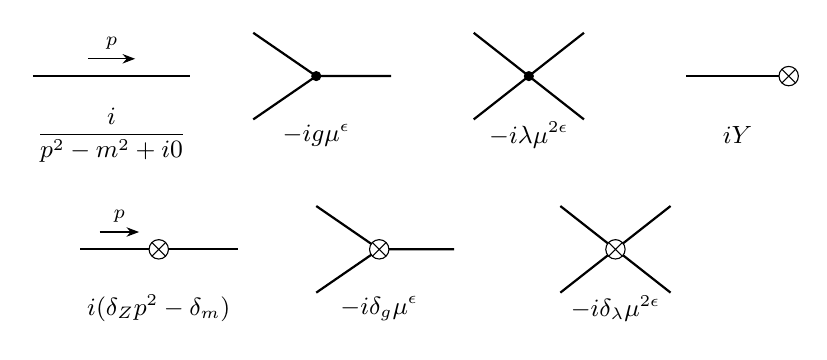
\begin{tikzpicture}
\begin{scope}[shift={(0,0)}]
  \draw[prop] (0,0) -- (2,0);
  \draw[mom] (0.7,0.22) -- (1.3,0.22) node[midway,above,font=\scriptsize] {$p$};
  \node[lab] at (1,-0.75) {$\dfrac{i}{p^2-m^2+i0}$};
\end{scope}
\begin{scope}[shift={(3.6,0)}]
  \draw[prop] (0,0) -- (-0.8,0.55) (0,0) -- (-0.8,-0.55) (0,0) -- (0.95,0);
  \node[vtx] at (0,0) {};
  \node[lab] at (0,-0.75) {$-ig\mu^{\epsilon}$};
\end{scope}
\begin{scope}[shift={(6.3,0)}]
  \draw[prop] (-0.7,0.55) -- (0.7,-0.55) (-0.7,-0.55) -- (0.7,0.55);
  \node[vtx] at (0,0) {};
  \node[lab] at (0,-0.75) {$-i\lambda\mu^{2\epsilon}$};
\end{scope}
\begin{scope}[shift={(8.3,0)}]
  \draw[prop] (0,0) -- (1.3,0);
  \node[ctv] at (1.3,0) {};
  \node[lab] at (0.65,-0.75) {$iY$};
\end{scope}
\begin{scope}[shift={(0.6,-2.2)}]
  \draw[prop] (0,0) -- (2,0);
  \node[ctv] at (1,0) {};
  \draw[mom] (0.25,0.22) -- (0.75,0.22) node[midway,above,font=\scriptsize] {$p$};
  \node[lab] at (1,-0.75) {$i(\delta_Zp^2-\delta_m)$};
\end{scope}
\begin{scope}[shift={(4.4,-2.2)}]
  \draw[prop] (0,0) -- (-0.8,0.55) (0,0) -- (-0.8,-0.55) (0,0) -- (0.95,0);
  \node[ctv] at (0,0) {};
  \node[lab] at (0,-0.75) {$-i\delta_g\mu^{\epsilon}$};
\end{scope}
\begin{scope}[shift={(7.4,-2.2)}]
  \draw[prop] (-0.7,0.55) -- (0.7,-0.55) (-0.7,-0.55) -- (0.7,0.55);
  \node[ctv] at (0,0) {};
  \node[lab] at (0,-0.75) {$-i\delta_\lambda\mu^{2\epsilon}$};
\end{scope}
\end{tikzpicture}
\caption{式~\eqref{eq:L} から導いた Feynman 則（\ref{app:rules}）。上の段は左から伝播関数、3点頂点、4点頂点、線形項。下の段は2点・3点・4点の対抗項。$\otimes$ は対抗項（と線形項）の挿入を表す。ループ運動量 $k$ ごとに $\int\dd^Dk/(2\pi)^D$ を掛け、対称性因子で割る。}
\label{fig:rules}
\end{figure}

\begin{figure}[tbp]
\centering
\begin{tikzpicture}
% row 1: V1, V2
\begin{scope}[shift={(0,0)}]
  \draw[prop] (-1.1,0) -- (0,0);
  \draw[prop] (0,0.5) circle (0.5);
  \node[vtx] at (0,0) {};
  \node[lab] at (0,-0.55) {(a) $V_1$：$g$};
  \node[lab,font=\footnotesize] at (0,-1.0) {$1/2$};
\end{scope}
\begin{scope}[shift={(4.2,0.3)}]
  \draw[prop] (-1.5,0) -- (-0.55,0) (0.55,0) -- (1.5,0);
  \draw[prop] (0,0) circle (0.55);
  \node[vtx] at (-0.55,0) {}; \node[vtx] at (0.55,0) {};
  \node[lab] at (0,-0.85) {(b) $V_2$：$g^2$};
  \node[lab,font=\footnotesize] at (0,-1.3) {$1/2$};
\end{scope}
\begin{scope}[shift={(8.6,0)}]
  \draw[prop] (-1.2,0) -- (1.2,0);
  \draw[prop] (0,0.5) circle (0.5);
  \node[vtx] at (0,0) {};
  \node[lab] at (0,-0.55) {(c) $V_2$：$\lambda$};
  \node[lab,font=\footnotesize] at (0,-1.0) {$1/2$};
\end{scope}
% row 2: V3
\begin{scope}[shift={(2.0,-2.9)}]
  \coordinate (A) at (-0.65,0); \coordinate (B) at (0.45,0.65); \coordinate (C) at (0.45,-0.65);
  \draw[prop] (A) -- (B) -- (C) -- cycle;
  \draw[prop] (A) -- (-1.4,0) (B) -- (1.05,1.1) (C) -- (1.05,-1.1);
  \node[vtx] at (A) {}; \node[vtx] at (B) {}; \node[vtx] at (C) {};
  \node[lab] at (0,-1.45) {(d) $V_3$：$g^3$};
  \node[lab,font=\footnotesize] at (0,-1.9) {$1$};
\end{scope}
\begin{scope}[shift={(7.4,-2.9)}]
  \draw[prop] (-0.55,0) -- (-1.25,0.6) (-0.55,0) -- (-1.25,-0.6) (0.55,0) -- (1.4,0);
  \draw[prop] (0,0) circle (0.55);
  \node[vtx] at (-0.55,0) {}; \node[vtx] at (0.55,0) {};
  \node[lab] at (0,-1.45) {(e) $V_3$：$g\lambda$（3通り）};
  \node[lab,font=\footnotesize] at (0,-1.9) {$1/2$};
\end{scope}
% row 3: V4
\begin{scope}[shift={(0.6,-6.0)}]
  \draw[prop] (-0.55,0) -- (-1.2,0.6) (-0.55,0) -- (-1.2,-0.6) (0.55,0) -- (1.2,0.6) (0.55,0) -- (1.2,-0.6);
  \draw[prop] (0,0) circle (0.55);
  \node[vtx] at (-0.55,0) {}; \node[vtx] at (0.55,0) {};
  \node[lab] at (0,-1.3) {(f) $V_4$：$\lambda^2$（3通り）};
  \node[lab,font=\footnotesize] at (0,-1.75) {$1/2$};
\end{scope}
\begin{scope}[shift={(5.0,-6.0)}]
  \coordinate (A) at (-0.6,0); \coordinate (B) at (0.5,0.65); \coordinate (C) at (0.5,-0.65);
  \draw[prop] (A) -- (B) -- (C) -- cycle;
  \draw[prop] (A) -- (-1.25,0.6) (A) -- (-1.25,-0.6) (B) -- (1.1,1.1) (C) -- (1.1,-1.1);
  \node[vtx] at (A) {}; \node[vtx] at (B) {}; \node[vtx] at (C) {};
  \node[lab] at (0,-1.3) {(g) $V_4$：$\lambda g^2$（6通り）};
  \node[lab,font=\footnotesize] at (0,-1.75) {$1$};
\end{scope}
\begin{scope}[shift={(9.4,-6.0)}]
  \draw[prop] (-0.55,-0.55) rectangle (0.55,0.55);
  \draw[prop] (-0.55,0.55) -- (-1.0,1.0) (0.55,0.55) -- (1.0,1.0) (-0.55,-0.55) -- (-1.0,-1.0) (0.55,-0.55) -- (1.0,-1.0);
  \node[vtx] at (-0.55,0.55) {}; \node[vtx] at (0.55,0.55) {}; \node[vtx] at (-0.55,-0.55) {}; \node[vtx] at (0.55,-0.55) {};
  \node[lab] at (0,-1.3) {(h) $V_4$：$g^4$（3通り）};
  \node[lab,font=\footnotesize] at (0,-1.75) {$1$};
\end{scope}
\end{tikzpicture}
\caption{1ループの1PI 図と、その対称性因子（\ref{app:rules}）。括弧は外線の付け方の数である。外線にタドポールが付いた図は線形項 $Y$ で打ち消すので含めない。}
\label{fig:oneloop}
\end{figure}

\paragraph{べき数え上げ。}外線 $E$ 本、3点頂点 $V_3$ 個、4点頂点 $V_4$ 個の図の表面的な発散次数は、$d=4$ で
\begin{equation}
\omega=4-E-V_3
\label{eq:omega}
\end{equation}
である（\ref{app:counting}）。4点頂点は発散次数を変えない。1ループの1PI 図では $V_3+2V_4=E$ なので、図~\ref{fig:oneloop} の (a)〜(h) の $\omega$ はそれぞれ $2,\,0,\,2,\,-2,\,0,\,0,\,-2,\,-4$ である。発散するのはタドポール、自己エネルギーの2種類、3点関数の $g\lambda$ の泡、4点関数の $\lambda^2$ の泡で、$g^3$ と $\lambda g^2$ の三角形、$g^4$ の箱は有限である。

\paragraph{1ループの1PI 関数。}1ループのスカラー積分を、$\phi^3$ のノートと同じく
\begin{equation}
I_N(q_1,\dots,q_N)\equiv\int\frac{\dd^Dk}{(2\pi)^D}\prod_{j=1}^{N}\frac{1}{(k+q_j)^2-m^2+i0}
\label{eq:IN}
\end{equation}
と定義する。図~\ref{fig:oneloop} の図を Feynman 則で書き、対抗項を加えると
\begin{equation}
\begin{aligned}
V_1&=iY+\frac{g\mu^\epsilon}{2}\,I_1,\\
V_2(p^2)&=\frac{g^2\mu^{2\epsilon}}{2}\,I_2(p^2)+\frac{\lambda\mu^{2\epsilon}}{2}\,I_1+i\bigl(\delta_Zp^2-\delta_m\bigr),\\
V_3&=g^3\mu^{3\epsilon}\,I_3+\frac{g\lambda\mu^{3\epsilon}}{2}\sum_{i=1}^{3}I_2(p_i^2)-i\,\delta_g\mu^{\epsilon},\\
V_4&=\frac{\lambda^2\mu^{4\epsilon}}{2}\sum_{x=s,t,u}I_2(x)+\lambda g^2\mu^{4\epsilon}\sum_{(6)}I_3+g^4\mu^{4\epsilon}\sum_{(3)}I_4-i\,\delta_\lambda\mu^{2\epsilon}
\end{aligned}
\label{eq:V}
\end{equation}
となる（\ref{app:ren}）。$V_3$ の和の $p_i$ は、図 (e) で3点頂点に付く外線の運動量である。$V_4$ の $\lambda g^2$ の和は4点頂点に付く外線の対の選び方6通り、$g^4$ の和は箱の外線の並べ方3通りについてとる。1ループで外線1本の図を4点頂点で作ることはできないので、$V_1$ は $\phi^3$ 理論と同じである。タドポールの条件 $V_1=0$ から $Y=(ig\mu^\epsilon/2)\,I_1$ と決まる。

\paragraph{$\overline{\mathrm{MS}}$ の対抗項。}$d=4$ で発散するのは $I_1$ と $I_2$ だけで、その極は $I_1|_{\mathrm{pole}}=im^2/((4\pi)^2\epsilon)$、$I_2|_{\mathrm{pole}}=i/((4\pi)^2\epsilon)$ である。$I_2$ の極は外運動量によらない（\ref{app:ren}）。式~\eqref{eq:V} の極が消えるように対抗項を決めると
\begin{equation}
\delta_Z=0,\qquad
\delta_m=\frac{g^2+\lambda m^2}{2(4\pi)^2}\,\Delta_{\mathrm{UV}},\qquad
\delta_g=\frac{3g\lambda}{2(4\pi)^2}\,\Delta_{\mathrm{UV}},\qquad
\delta_\lambda=\frac{3\lambda^2}{2(4\pi)^2}\,\Delta_{\mathrm{UV}}
\label{eq:ct}
\end{equation}
を得る。$\delta_m$ の $g^2$ の項は $\phi^3$ 理論と同じで、$\lambda m^2$ の項は図 (c) から来る。$\delta_g$ は図 (e) の3つの泡の、$\delta_\lambda$ は図 (f) の3つの泡の極を打ち消す。1ループの自己エネルギーの極は $p^2$ によらないので、$\delta_Z=0$ である。

\paragraph{繰り込まれた1PI 関数。}式~\eqref{eq:ct} を式~\eqref{eq:V} に入れて $\epsilon\to0$ とすると
\begin{equation}
\begin{aligned}
V_2&=\frac{i}{2(4\pi)^2}\bigl[g^2B_0(p^2)+\lambda A_0(m^2)\bigr],\qquad
V_3=\frac{i}{(4\pi)^2}\Bigl[g^3C_0+\frac{g\lambda}{2}\sum_{i=1}^3B_0(p_i^2)\Bigr],\\
V_4&=\frac{i}{(4\pi)^2}\Bigl[\frac{\lambda^2}{2}\sum_{x=s,t,u}B_0(x)+\lambda g^2\sum_{(6)}C_0+g^4\sum_{(3)}D_0\Bigr]
\end{aligned}
\label{eq:VR}
\end{equation}
となる（\ref{app:ren}）。$A_0(m^2)=m^2\bigl(1-\ln(m^2/\mu^2)\bigr)$、$B_0(p^2)=-\int_0^1\dd x\,\ln[(m^2-x(1-x)p^2-i0)/\mu^2]$、$C_0=-\int\dd F\,\Delta^{-1}$ は $\phi^3$ のノートと同じ $\overline{\mathrm{MS}}$ の有限部分で、$D_0=\int\dd F\,\Delta^{-2}$ は有限な箱の積分である。どれも LoopTools の規約（$\Delta=0$）の値と同じである。自己エネルギーは $\Sigma\equiv iV_2=-[g^2B_0(p^2)+\lambda A_0(m^2)]/(2(4\pi)^2)$ で、$\lambda A_0$ の項は運動量によらず、質量をずらすだけである。

\paragraph{繰り込み群。}裸の量 $m_0^2=m^2+\delta_m$、$g_0=\mu^\epsilon(g+\delta_g)$、$\lambda_0=\mu^{2\epsilon}(\lambda+\delta_\lambda)$ が $\mu$ によらないことから
\begin{equation}
\beta_\lambda=\frac{3\lambda^2}{(4\pi)^2},\qquad
\beta_g=\frac{3g\lambda}{(4\pi)^2},\qquad
\gamma\equiv\mu\frac{\dd m^2}{\dd\mu}=\frac{g^2+\lambda m^2}{(4\pi)^2}
\label{eq:rge}
\end{equation}
を得る（\ref{app:rg}）。$\delta_Z=0$ なので、1ループでは場の異常次元は0である。$\beta_\lambda$ は $\lambda\phi^4$ 理論のよく知られた値で、$\lambda$ は高エネルギーで大きくなる。$\gamma$ の $g^2$ の項は、$\phi^3$ 理論の質量の走りと同じである。同じ三つの係数は、1ループの有効ポテンシャル（Coleman--Weinberg ポテンシャル~\cite{cw}）の $\mu$ 依存を、ポテンシャルの係数の走りで打ち消す条件からも得られる（\ref{app:rg}）。$\beta_g$ には $g$ の自乗の項がなく、$\lambda$ に比例する。$\lambda=0$ なら $g$ は走らない（$\phi^3$ 理論と同じ）。

\paragraph{木レベルの散乱振幅。}$\phi\phi\to\phi\phi$ の木の振幅は、$s,t,u$ の3つのチャンネルと接触項の和
\begin{equation}
\mathcal{M}^{(0)}=-g^2\left[\frac{1}{s-m^2}+\frac{1}{t-m^2}+\frac{1}{u-m^2}\right]-\lambda
\label{eq:Mtree}
\end{equation}
である（図~\ref{fig:tree}、\ref{app:tree}）。各図の対称性因子は1である。

\begin{figure}[tbp]
\centering
\begin{tikzpicture}
\begin{scope}[shift={(0,0)}]
  \draw[prop] (-1.1,0.6) -- (-0.45,0) -- (-1.1,-0.6) (1.1,0.6) -- (0.45,0) -- (1.1,-0.6) (-0.45,0) -- (0.45,0);
  \node[vtx] at (-0.45,0) {}; \node[vtx] at (0.45,0) {};
  \node[lab] at (0,-1.0) {$s$};
\end{scope}
\begin{scope}[shift={(3.4,0)}]
  \draw[prop] (-0.8,0.8) -- (0,0.4) -- (0.8,0.8) (-0.8,-0.8) -- (0,-0.4) -- (0.8,-0.8) (0,0.4) -- (0,-0.4);
  \node[vtx] at (0,0.4) {}; \node[vtx] at (0,-0.4) {};
  \node[lab] at (0,-1.0) {$t$};
\end{scope}
\begin{scope}[shift={(6.6,0)}]
  \draw[prop] (-0.8,0.8) -- (0,0.4) (0,0.4) -- (0.8,-0.8) (-0.8,-0.8) -- (0,-0.4) (0,-0.4) -- (0.8,0.8) (0,0.4) -- (0,-0.4);
  \node[vtx] at (0,0.4) {}; \node[vtx] at (0,-0.4) {};
  \node[lab] at (0,-1.0) {$u$};
\end{scope}
\begin{scope}[shift={(9.6,0)}]
  \draw[prop] (-0.8,0.6) -- (0.8,-0.6) (-0.8,-0.6) -- (0.8,0.6);
  \node[vtx] at (0,0) {};
  \node[lab] at (0,-1.0) {接触項};
\end{scope}
\end{tikzpicture}
\caption{$\phi\phi\to\phi\phi$ の木の図。3点頂点2つの $s,t,u$ チャンネルと、4点頂点1つの接触項。}
\label{fig:tree}
\end{figure}
\paragraph{1ループの $\phi\phi\to\phi\phi$ 振幅。}1ループの振幅（外線の補正を除き、タドポールは $Y$ で打ち消す）は、1PI の4点関数 $V_4$ と、木の $s,t,u$ チャンネルの図の両端の頂点に $V_3$ を付けた図、内線に $V_2$ を付けた図の和である（\ref{app:scat}）。$\overline{\mathrm{MS}}$ で繰り込むと
\begin{equation}
\begin{aligned}
(4\pi)^2\,\mathcal{M}^{(1)}={}&g^4\Bigl[\sum D_0+\sum_x\Bigl(\frac{2C_0(x)}{x-m^2}+\frac{B_0(x)}{2(x-m^2)^2}\Bigr)\Bigr]\\
&+g^2\lambda\sum_x\Bigl[2C_0(x)+\frac{B_0(x)+2B_0(m^2)}{x-m^2}+\frac{A_0(m^2)}{2(x-m^2)^2}\Bigr]+\frac{\lambda^2}{2}\sum_xB_0(x)
\end{aligned}
\label{eq:M1}
\end{equation}
となる。和は $x=s,t,u$ についてとり、$C_0(x)\equiv C_0(m^2,m^2,x)$、$\sum D_0\equiv D_0(s,t)+D_0(s,u)+D_0(t,u)$ である（外線はすべて質量殻上、内線の質量はすべて $m$）。$\lambda=0$ とすると $\phi^3$ のノートの1ループの振幅（同ノートの式 (17)）に戻る。$g^2\lambda$ の項は、$V_4$ の $\lambda g^2$ の三角形（$2C_0$）、頂点補正の $g\lambda$ の泡（$B_0(x)+2B_0(m^2)$）、内線の自己エネルギーの $\lambda$ の図（$A_0$）から来る。$\lambda^2$ の項は $V_4$ の泡だけである。虚部は $s$ チャンネルのユニタリー性
\begin{equation}
\mathrm{Im}\,\mathcal{M}^{(1)}(s,t)=\frac14\,\frac{p}{16\pi^2\sqrt s}\int\!\dd\Omega_k\,\mathcal{M}^{(0)}(s,t_1)\,\mathcal{M}^{(0)}(s,t_2)
\label{eq:unit}
\end{equation}
を満たす（\ref{app:scat}）。$p$ は重心系の運動量、$k$ は中間状態の一方の粒子の運動量で、$t_1=(p_1-k)^2$、$t_2=(k_1-k)^2$ である。前方 $t=0$ では、これは光学定理 $\mathrm{Im}\,\mathcal{M}^{(1)}(s,0)=2p\sqrt s\,\sigma$ になる。


\paragraph{真空の構造。}式~\eqref{eq:L} のポテンシャル $V(\phi)=\frac12m^2\phi^2+\frac{g}{3!}\phi^3+\frac{\lambda}{4!}\phi^4$ は、$\phi=(m^2/g)f$ と置くと
\begin{equation}
V=\frac{m^6}{g^2}\Bigl(\frac12f^2+\frac16f^3+\frac{\alpha}{72}f^4\Bigr),\qquad
\alpha\equiv\frac{3\lambda m^2}{g^2}
\label{eq:vac}
\end{equation}
となり、ポテンシャルの形は一つの数 $\alpha$ だけで決まる（\ref{app:vacuum}）。$\alpha>9/8$ では $\phi=0$ が唯一の極小である。$\alpha<9/8$ では、$f_-=-\frac{9}{2\alpha}\bigl(1+\sqrt{1-8\alpha/9}\bigr)$ に二つ目の極小が現れる（$g>0$ のとき）。$1<\alpha<9/8$ ではそれは $\phi=0$ より高く、$\alpha=1$ で二つの極小が縮退し、$\alpha<1$ では二つ目の極小のほうが低くなって $\phi=0$ が偽の真空になる。$\alpha\to0$ は $\phi^3$ 理論で、二つ目の極小は無限遠に去り、ポテンシャルは下に有界でなくなる。Dunne と Min~\cite{dunnemin}、Dine ら~\cite{dine92} が bounce と前因子を調べたポテンシャル $\frac12\Phi^2-\frac12\Phi^3+\frac\alpha8\Phi^4$ は、$\Phi=-f/3$ とすると式~\eqref{eq:vac} の括弧の $1/9$ になる。その $\alpha$ は本ノートの $\alpha$ と同じである。

SM のヒッグスのポテンシャル $\lambda_{\mathrm{SM}}(H^\dagger H-v^2/2)^2$ をユニタリーゲージで展開すると、$V=\frac12m_h^2h^2+\frac{m_h^2}{2v}h^3+\frac{m_h^2}{8v^2}h^4$ である（$m_h^2=2\lambda_{\mathrm{SM}}v^2$）。3点と4点の結合を $\kappa_3$、$\kappa_4$ 倍すると、本ノートの記号では
\begin{equation}
g=\kappa_3\,\frac{3m_h^2}{v},\qquad\lambda=\kappa_4\,\frac{3m_h^2}{v^2},\qquad\alpha=\frac{\kappa_4}{\kappa_3^2}
\label{eq:kappa}
\end{equation}
となる。SM（$\kappa_3=\kappa_4=1$）はちょうど $\alpha=1$ にあたり、縮退した二つの極小は $h=0$ と $h=-2v$ である。SM ではこの二つは $H\to-H$ のゲージ変換で移り合う同じ真空だが、場が一つの本模型では別の真空になる。4点結合を SM の値に保って3点結合だけを大きくすると（$\kappa_3>1$）$\alpha<1$ となり、$h=0$ は偽の真空になる。したがって、この模型の偽の真空の崩壊は、$\kappa_3$ と $\kappa_4$ の限界に読み替えられる。

\section{検算の計画}\label{sec:plan}

第~\ref{sec:results} 節の各量を、どの手段で計算して突き合わせるかを表~\ref{tab:plan} に示す。手計算（付録）を基準とし、ツールの出力がそれと一致するかを確かめる。ツールの版と配置は計算環境の記録~\cite{env} にあり、$\phi^3$ のノートで使ったものと同じである。

\begin{table}[tbp]
\centering\small
\caption{各量と、それを計算して突き合わせる手段。「—」はその手段を使わないこと、「今後」は手計算をこれから付録に加えることを表す。}
\label{tab:plan}
\begin{tabularx}{\linewidth}{>{\raggedright\arraybackslash}p{3.4cm}>{\raggedright\arraybackslash}p{1.6cm}>{\raggedright\arraybackslash}X>{\raggedright\arraybackslash}p{2.0cm}>{\raggedright\arraybackslash}p{1.7cm}>{\raggedright\arraybackslash}p{2.0cm}}
\toprule
\textbf{量} & \textbf{手計算} & \textbf{FeynCalc（+ FeynArts）} & \textbf{Package-X} & \textbf{LoopTools、COLLIER} & \textbf{MadGraph} \\
\midrule
Feynman 則・対称性因子 & \ref{app:rules} & 書き出した FeynArts 模型の係数と、図の対称性因子 & — & — & UFO の頂点と図の数 \\
木の振幅 \eqref{eq:Mtree} & \ref{app:tree} & 記号として一致 & — & — & 断面積 \\
1PI 関数の極と対抗項 \eqref{eq:ct} & \ref{app:ren} & PaVe 関数に簡約し、極を抽出 & 解析式 & — & — \\
1PI 関数の有限部分 \eqref{eq:VR} & \ref{app:ren} & 対抗項を加える & 解析式 & 数値 & — \\
1ループの $\phi\phi\to\phi\phi$ \eqref{eq:M1} と S 行列要素 & \ref{app:scat}、S 行列要素は今後 & 記号として比べる（FormCalc でも） & 数値 & 数値 & MadLoop \\
全断面積（$2\to3$ を含む） & 今後 & — & — & COLLIER & MadLoop、$2\to3$ \\
繰り込み群 \eqref{eq:rge} & \ref{app:rg} & $\mu$ を変えて評価 & 数値 & 数値 & MadLoop の $\mu_R$ \\
\bottomrule
\end{tabularx}
\end{table}

\paragraph{一致の基準。}発散部分と対抗項は、$1/\epsilon$ の係数が記号として完全に一致することを求める。有限部分は、基準点で、ツールどうしと手計算の数値が倍精度の丸め誤差の範囲（相対 $10^{-12}$ 程度）で一致することを求める。FeynCalc の PaVe 関数の $\epsilon^0$ の係数は $\overline{\mathrm{MS}}$ の値から $-(\gamma_E+\ln\pi)$ だけずれるので、$\phi^3$ のノートと同じく本ノートの $V_n$ に直してから比べる。MadGraph の断面積は、自分で数値積分した値と統計誤差の範囲で一致することを求める。

\paragraph{手順。}次の順に進める。(1) 模型ファイル \texttt{Phi34.fr} を作り、FeynArts の模型と UFO を書き出して、Feynman 則と MadGraph の図を確かめる。(2) 木の振幅を FeynCalc と MadGraph で確かめる。(3) 1ループの1PI 関数（2点〜4点）の極と対抗項を FeynCalc・Package-X で確かめ、有限部分を Package-X・LoopTools・COLLIER で比べる。(4) 1ループの $\phi\phi\to\phi\phi$ を FeynCalc と FormCalc の二つの経路で求め、数値をツールどうしで比べ、虚部をユニタリー性で確かめる。(5) 極質量と留数で S 行列要素に直し、NLOCT で作った UFO の MadLoop と比べる。(6) 全断面積を、1ループの補正と $\phi\phi\to\phi\phi\phi$（図25個）を含めて求める。(7) S 行列要素の $\mu$ 依存から $\beta_\lambda$、$\beta_g$、$\gamma$ を同時に読み取り、式~\eqref{eq:rge} と比べ、繰り込み群の流れを描く。(8) 部分波のユニタリー性から、$(g/m,\lambda)$、すなわち $(\kappa_3,\kappa_4)$ の限界を出す。(9) 偽の真空の bounce の作用を $d=4$ と $d=3$ で $\alpha$ の関数として求め、$d=3$ を Dine ら~\cite{dine92} と照合する。(10) $d=4$ の崩壊率の1ループの前因子を $\alpha$ の関数として求め、Dunne と Min~\cite{dunnemin} と照合し、$(\kappa_3,\kappa_4)$ の真空の安定性の限界を出す。

\section{1ループの量と散乱の検算}\label{sec:checks}

第~\ref{sec:plan} 節の手順を順に行う。現在は手順 (4) まで終わっている。スクリプトはすべて \texttt{Src/} にあり、手順 (1) は \texttt{run\_model\_check.sh} で、手順 (2) は \texttt{run\_tree\_check.sh} で、手順 (3) は \texttt{run\_oneloop\_check.sh} で、手順 (4) は \texttt{run\_scat\_check.sh} で再実行できる。

\paragraph{手順 (1)：模型ファイル。}FeynRules の模型ファイル \texttt{Src/Phi34.fr} を作った。ラグランジアンは式~\eqref{eq:L} から対抗項と線形項を除いた部分である。$\phi^3$ のノートと同じく、3点結合は \texttt{gphi}（\texttt{g} という名前は FeynRules の UFO 出力を止めるため）と書き、4点結合は \texttt{lamphi} と書いた。MadGraph の結合の次数は、\texttt{gphi} を \texttt{PHI}$=1$、\texttt{lamphi} を \texttt{PHI}$=2$ と数える。$\lambda$ は $g^2/m^2$ と同じ次数なので、\texttt{PHI} が2増えるごとにループの次数が一つ上がる。FeynRules のチェック（エルミート性、運動項の規格化、質量スペクトル）はすべて通った。頂点は $-i\,\texttt{gphi}$ と $-i\,\texttt{lamphi}$ になり、図~\ref{fig:rules} の $-ig$、$-i\lambda$ と一致した。FeynArts 模型（\texttt{C[S[1],S[1],S[1]]} と \texttt{C[S[1],S[1],S[1],S[1]]}）と UFO も \texttt{Src/generated/} に書き出せた。MadGraph 3.8.1 はその UFO から、$\phi\phi\to\phi\phi$ の図を4つ（$s,t,u$ と接触項、図~\ref{fig:tree}）、$\phi\phi\to\phi\phi\phi$ の図を25個生成した。25個は、3点頂点3つの図15個（$\phi^3$ 理論と同じ）と、3点頂点と4点頂点を1つずつ持つ図10個（4点頂点に付く外線3本の選び方 $\binom53=10$）である。スクリプトは \texttt{generate\_Phi34.wl}（FeynRules）と \texttt{model\_mg5.mg5}（MadGraph）である。

\paragraph{手順 (2)：木の振幅。}\texttt{Src/generated/Phi34\_FA} の FeynArts 模型から $\phi\phi\to\phi\phi$ の木の図を作ると、$s,t,u$ の3つと接触項の計4つが対称性因子 $1$ で現れた。FeynCalc で振幅を組み立てて Mandelstam 変数で書くと、式~\eqref{eq:Mtree} との差は記号として $0$ になった。数値でも、$\sqrt s=5$、$\cos\theta=0.3$、$m=g=\lambda=1$ で $\mathcal{M}^{(0)}=-0.8536468020$ となり、式~\eqref{eq:Mtree} を Python で評価した値と一致した。これは $\phi^3$ のノートの同じ点の値 $0.1463531980$ から $\lambda=1$ を引いたものである。

続いて、UFO を MadGraph 3.8.1 に読み込ませ、固定エネルギーの $\phi$ どうしの衝突で全断面積を求めた。カットはかけず、$m=g=\lambda=1$（単位は GeV）とした。比べる相手は、式~\eqref{eq:Mtree} の $|\mathcal{M}^{(0)}|^2$ を角度について数値積分した
\begin{equation}
\sigma=\frac12\int\!\dd\Omega\,\frac{|\mathcal{M}^{(0)}|^2}{64\pi^2s},\qquad
t=-2p^2(1-\cos\theta),\quad u=-2p^2(1+\cos\theta),\quad p^2=\frac s4-m^2
\label{eq:sigma}
\end{equation}
である（導出は $\phi^3$ のノートの付録~F と同じ）。因子 $\frac12$ は、終状態の二つの $\phi$ が同種粒子であることから来る。表~\ref{tab:tree} に示すように、$\sqrt s=2.5,\,5,\,10$ のすべてで、MadGraph の値は式~\eqref{eq:sigma} と統計誤差の0.84倍以内で一致した。$\lambda$ の接触項は、閾値の近くでは $\phi^3$ の振幅と逆符号で打ち消し合い、$\sqrt s=2.5$ の断面積を $\phi^3$ 理論の約 $1/24$ にする。高いエネルギーでは $\phi^3$ の振幅が $1/s$ のように小さくなるので、接触項が振幅の大部分を占め、$\sqrt s=10$ の断面積は $\phi^3$ 理論の約41倍になる。スクリプトは \texttt{tree\_feyncalc.wl}（FeynCalc）、\texttt{tree\_mg5.mg5}（MadGraph）、\texttt{tree\_sigma.py}（数値積分と比較）である。

\begin{table}[tbp]
\centering\small
\caption{$\phi\phi\to\phi\phi$ の木の全断面積（$m=g=\lambda=1$、単位は GeV、$1~\mathrm{GeV}^{-2}=0.3893794\times10^{9}$~pb）。「解析式」は式~\eqref{eq:sigma} の数値積分（相対精度 $10^{-12}$）、MadGraph の誤差はモンテカルロ積分の統計誤差である。}
\label{tab:tree}
\begin{tabular}{rrrr}
\toprule
$\sqrt{s}$ [GeV] & 解析式 [pb] & MadGraph [pb] & 差／誤差 \\
\midrule
2.5 & $1.92995\times10^{4}$ & $(1.9320\pm0.0031)\times10^{4}$ & $0.67$ \\
5 & $9.11410\times10^{4}$ & $(9.1220\pm0.0094)\times10^{4}$ & $0.84$ \\
10 & $3.29352\times10^{4}$ & $(3.2960\pm0.0038)\times10^{4}$ & $0.65$ \\
\bottomrule
\end{tabular}
\end{table}

\paragraph{手順 (3)：1ループの1PI 関数。}三つの観点から確かめた。まず図と振幅である。\texttt{Src/generated/Phi34\_FA} から FeynArts で1PI 図を作ると、$V_1$ が1つ、$V_2$ が2つ、$V_3$ が4つ、$V_4$ が12個現れ、図~\ref{fig:oneloop} と一致した。$V_4$ では、1粒子既約でない位相（\texttt{Reducible}）を除いた。除かないと、木の図に自己エネルギーや頂点補正を付けた図も含めて42個になる。FeynCalc でテンソル積分を PaVe 関数まで簡約すると、四つの振幅は式~\eqref{eq:V} に $(2\pi)^D$ を掛けたものと記号として一致した。外線が質量殻上のとき、$V_4$ の $\lambda g^2$ の6つの三角形は、各チャンネル $x=s,t,u$ について $C_0(m^2,m^2,x)$ が2つずつになる。

次に発散部分である。Package-X で $V_n$ の $1/\epsilon$ の係数を取り出すと、$V_1$ が $igm^2/(2(4\pi)^2)$、$V_2$ が $i(g^2+\lambda m^2)/(2(4\pi)^2)$、$V_3$ が $3ig\lambda/(2(4\pi)^2)$、$V_4$ が $3i\lambda^2/(2(4\pi)^2)$ だった。極を消す条件から決めた $\overline{\mathrm{MS}}$ の対抗項は、式~\eqref{eq:ct} と記号として一致した。

最後に有限部分を、$m=\mu=g=\lambda=1$ で式~\eqref{eq:VR} の括弧 $b_n\equiv(4\pi)^2V_n/i$ として比べた（表~\ref{tab:oneloop}）。Package-X と LoopTools は FeynCalc の振幅を評価し、COLLIER は式~\eqref{eq:VR} を組み立てた。$b_2$ は $B_0$ の閉じた式（$\phi^3$ のノートの付録~G）とも比べた。$V_2$ の6点、$V_3$ の5点、$V_4$ の6点（$\sqrt s=2.5,\,5,\,10$、$\cos\theta=0.3,\,0.9$）で、三つのツールは相対 $1.4\times10^{-11}$ 以内で一致した。最大のずれは $\sqrt s=2.5$ の $V_4$ の Package-X で、$\phi^3$ のノートでも見た、Package-X の $D_0$ の数値関数の精度の限界である。LoopTools と COLLIER は相対 $2\times10^{-15}$ 以内で一致した。ただし、外運動量の2乗がすべて負で互いに異なる点 $(k_1^2,k_2^2,p^2)=(-1,-2,-3)$ では、LoopTools の $C_0$ が FF のエラーを出し、全く違う値を返した。Package-X と COLLIER は、この点で相対 $3\times10^{-15}$ で一致した。スクリプトは \texttt{oneloop\_feyncalc.wl}（FeynCalc、Package-X、LoopTools）、\texttt{oneloop\_collier.f90}（COLLIER）、\texttt{oneloop\_numeric.py}（比較）である。

\begin{table}[tbp]
\centering\small
\caption{1ループの1PI 関数の有限部分（$m=\mu=g=\lambda=1$）。$b_n\equiv(4\pi)^2V_n/i$ は式~\eqref{eq:VR} の括弧である。基準値は COLLIER（$b_2$ は $B_0$ の閉じた式）で、右の2列は基準値に対する相対的なずれである。$V_3$ の点は $(k_1^2,k_2^2,p^2)$、$V_4$ の点は $(\sqrt s,\cos\theta)$ である。×は LoopTools が誤った値を返した点を表す。}
\label{tab:oneloop}
\begin{tabular}{llrrrr}
\toprule
関数 & 点 & $\mathrm{Re}\,b_n$ & $\mathrm{Im}\,b_n$ & Package-X & LoopTools \\
\midrule
$V_2$ & $p^2=-5$〜$10$ の6点 & — & — & $0$ & $1.3\times10^{-15}$ \\
\midrule
$V_3$ & $(1,1,-5)$ & $-0.538265452328$ & $0$ & $2.7\times10^{-15}$ & $7.3\times10^{-16}$ \\
 & $(1,1,-1)$ & $-0.444564270555$ & $0$ & $2.6\times10^{-13}$ & $7.7\times10^{-16}$ \\
 & $(1,1,5)$ & $-0.075778938873$ & $-0.271364631851$ & $7.8\times10^{-13}$ & $1.9\times10^{-15}$ \\
 & $(1,1,10)$ & $0.182470663658$ & $0.427515514002$ & $1.1\times10^{-15}$ & $1.7\times10^{-16}$ \\
 & $(-1,-2,-3)$ & $-0.751035363817$ & $0$ & $3.3\times10^{-15}$ & ×\ $14$ \\
\midrule
$V_4$ & $(2.5,\,0.3)$ & $-2.681618902000$ & $-0.001524734291$ & $1.1\times10^{-12}$ & $1.2\times10^{-15}$ \\
 & $(2.5,\,0.9)$ & $-2.678096217617$ & $0.009355084748$ & $1.4\times10^{-11}$ & $1.8\times10^{-15}$ \\
 & $(5,\,0.3)$ & $-2.711728398837$ & $0.704674623333$ & $1.6\times10^{-15}$ & $7.9\times10^{-17}$ \\
 & $(5,\,0.9)$ & $-2.770596811313$ & $0.742698735099$ & $4.6\times10^{-14}$ & $8.1\times10^{-16}$ \\
 & $(10,\,0.3)$ & $-3.876301894467$ & $1.256255517211$ & $6.6\times10^{-15}$ & $3.4\times10^{-16}$ \\
 & $(10,\,0.9)$ & $-3.831926991172$ & $1.267382372518$ & $1.4\times10^{-14}$ & $5.4\times10^{-16}$ \\
\bottomrule
\end{tabular}
\end{table}

\paragraph{手順 (4)：1ループの $\phi\phi\to\phi\phi$。}二つの独立な経路で振幅を作った。一つは FeynCalc 用にパッチを当てた FeynArts と FeynCalc、もう一つはパッチを当てない FeynArts と FormCalc である。どちらでも図は42個（1PI が12個、頂点補正が24個、内線の自己エネルギーが6個）で、振幅は式~\eqref{eq:M1} と記号として一致した。FeynCalc の振幅の極は、式~\eqref{eq:ct} の三つの対抗項を木の図に入れた分 $-\sum_x[g^2\delta_m/(x-m^2)^2+2g\delta_g/(x-m^2)]-\delta_\lambda$ とちょうど打ち消し合った。FormCalc では LoopTools の $\Delta$ を0と1にして、$\Delta$ 依存がこの対抗項の係数とちょうど等しいことを確かめた。

数値は、$\phi^3$ のノートと同じ6点（$\sqrt s=2.5,\,5,\,10$、$\cos\theta=0.3,\,0.9$、$m=g=\lambda=\mu=1$）で、四つの経路（FeynCalc と Package-X、FeynCalc と LoopTools、FormCalc と LoopTools、COLLIER）で比べた（表~\ref{tab:scat}、図~\ref{fig:scat}）。実部は、COLLIER に対して LoopTools と FormCalc が相対 $5\times10^{-15}$ 以内、Package-X が $3.5\times10^{-12}$ 以内で一致した。虚部は、四つの経路すべてが式~\eqref{eq:unit} の2重積分（20桁）と相対 $4\times10^{-14}$ 以内で一致した。式~\eqref{eq:unit} の積分は、前方では式~\eqref{eq:sigma} から計算した $2p\sqrt s\,\sigma$ とも一致した。$g=\lambda=m=1$ では、$|\mathcal{M}^{(1)}|$ は $|\mathcal{M}^{(0)}|$ の $2$〜$4\%$ である。ただし $\sqrt s=2.5$、$\cos\theta=0.9$ では、手順 (2) で見た $\phi^3$ の振幅と接触項の打ち消し合いのために $\mathcal{M}^{(0)}=0.027$ と小さく、比は $26\%$ になる。スクリプトは \texttt{scat\_feyncalc.wl}（FeynCalc）、\texttt{scat\_formcalc.wl}（FormCalc）、\texttt{scat\_collier.f90}（COLLIER）、\texttt{scat\_numeric.py}（比較とユニタリー性）である。

\begin{table}[tbp]
\centering\small
\caption{1ループの $\phi\phi\to\phi\phi$ 振幅（式~\eqref{eq:M1}、$\overline{\mathrm{MS}}$、$m=g=\lambda=\mu=1$）。$\mathrm{Re}\,\mathcal{M}^{(1)}$ は COLLIER の値、$\mathrm{Im}\,\mathcal{M}^{(1)}$ は式~\eqref{eq:unit} の積分の値である。右の3列は相対的なずれで、「LT・FC」は LoopTools（FeynCalc 経由）と FormCalc と LoopTools の大きい方、「虚部」は Package-X・LoopTools・FormCalc・COLLIER の最大値である。}
\label{tab:scat}
\begin{tabular}{rrrrrrrr}
\toprule
$\sqrt s/m$ & $\cos\theta$ & $\mathcal{M}^{(0)}$ & $10^3\,\mathrm{Re}\,\mathcal{M}^{(1)}$ & $10^3\,\mathrm{Im}\,\mathcal{M}^{(1)}$ & 実部：Package-X & 実部：LT・FC & 虚部 \\
\midrule
2.5 & 0.3 & $-0.224944$ & $-9.66650729$ & $0.09844428$ & $8.5\times10^{-13}$ & $2.2\times10^{-15}$ & $3.8\times10^{-14}$ \\
2.5 & 0.9 & $0.027125$ & $-6.93898622$ & $0.16734154$ & $3.5\times10^{-12}$ & $4.7\times10^{-15}$ & $2.5\times10^{-14}$ \\
5 & 0.3 & $-0.853647$ & $-15.78556592$ & $5.01430785$ & $4.4\times10^{-15}$ & $4.4\times10^{-16}$ & $5.2\times10^{-16}$ \\
5 & 0.9 & $-0.506129$ & $-13.79834855$ & $5.25509835$ & $3.6\times10^{-14}$ & $6.3\times10^{-16}$ & $2.0\times10^{-15}$ \\
10 & 0.3 & $-0.965426$ & $-24.12031038$ & $8.13445335$ & $9.8\times10^{-15}$ & $4.3\times10^{-16}$ & $6.4\times10^{-16}$ \\
10 & 0.9 & $-0.826841$ & $-23.01487753$ & $8.20491498$ & $1.1\times10^{-14}$ & $4.5\times10^{-16}$ & $1.1\times10^{-15}$ \\
\bottomrule
\end{tabular}
\end{table}

\begin{figure}[tbp]
\centering
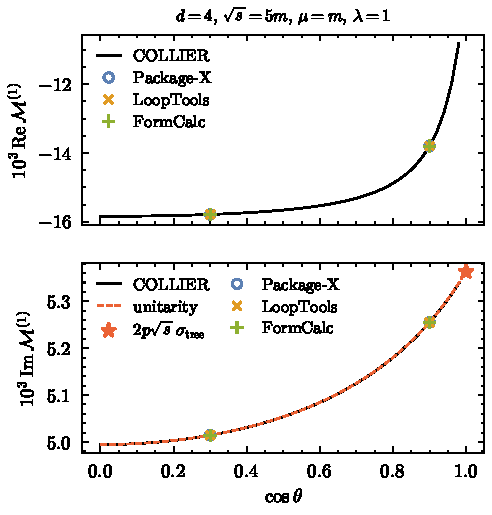
\includegraphics[width=0.6\linewidth]{../figs/scat_d4.pdf}
\caption{$\sqrt s=5m$ での $\mathcal{M}^{(1)}$ の実部（上）と虚部（下）の角度依存（$\overline{\mathrm{MS}}$、$m=g=\lambda=\mu=1$）。$\mathcal{M}^{(1)}$ は $\cos\theta\to-\cos\theta$（$t\leftrightarrow u$）で対称なので、$\cos\theta\ge0$ だけを示す。実線は COLLIER の積分から組み立てた式~\eqref{eq:M1}、記号は Package-X・LoopTools（FeynCalc 経由）・FormCalc と LoopTools の値、下の破線は式~\eqref{eq:unit}、星印は光学定理の値 $2p\sqrt s\,\sigma$ である。}
\label{fig:scat}
\end{figure}

\section{議論と今後}\label{sec:discussion}

\paragraph{処方についての注意。}本ノートは、$\phi^3$ のノートと同じく、タドポールを線形項 $Y$ で打ち消す処方をとる。この処方の $\beta_g$ と $\gamma$ は、対称な $\lambda\phi^4$ 理論を破れた真空のまわりで展開し、タドポールを打ち消さない処方とは異なる（\ref{app:rg}）。物理量はどちらの処方でも同じだが、文献の値とパラメータを比べるときは、処方の違いに注意が要る。

\paragraph{ツールの問題。}手順 (3) で、LoopTools の $C_0$ が、外運動量の2乗がすべて負で互いに異なる点 $(-1,-2,-3)$ で、FF のエラーとともに全く違う値を返すことが分かった。$\phi^3$ のノートでは、閾値より下で外運動量が0でない点（例えば $C_0(m^2,m^2,m^2)$）での誤りを見つけている。今回の点はそれとは別の領域である。当面、$C_0$ の基準には Package-X と COLLIER を使う。

\paragraph{今後。}第~\ref{sec:plan} 節の手順 (5) から順に進める。手順 (5) 以降の手計算（S 行列要素、全断面積、部分波、bounce と前因子）は、進めるにつれて付録に加える。

\appendix

\section{Feynman 則と対称性因子の導出}\label{app:rules}

\paragraph{伝播関数と頂点。}伝播関数 $i/(p^2-m^2+i0)$ と線形項 $iY$、2点の対抗項 $i(\delta_Zp^2-\delta_m)$、3点の頂点と対抗項 $-ig\mu^\epsilon$、$-i\delta_g\mu^\epsilon$ の導出は $\phi^3$ のノート~\cite{phi3note} の付録~A と同じである。4点の頂点は、相互作用 $\mathcal{L}\supset-(\lambda\mu^{2\epsilon}/4!)\phi^4$ から決まる。頂点の因子は「$i\times(\mathcal{L}_{\mathrm{int}}$ の係数$)\times($同種の場の付け方の数$)$」で、4点頂点では区別できる4本の線を4つの $\phi$ に付ける方法が $4!$ 通りあるので、$i\cdot(-\lambda\mu^{2\epsilon}/4!)\cdot4!=-i\lambda\mu^{2\epsilon}$ となる。4点の対抗項も同じく $-i\delta_\lambda\mu^{2\epsilon}$ である。

\paragraph{対称性因子の数え方。}図の値は、$\langle\phi\cdots\phi\,\frac{1}{n!}(i\int\mathcal{L}_{\mathrm{int}})^n\rangle$ の Wick の縮約のうち、その図を与えるものの数を、頂点の係数とともに数えて決める。同じ種類の頂点が $n$ 個あると $1/n!$ が付くが、どの頂点をどこに置くかの入れ替え $n!$ と打ち消す。以下、頂点の係数を $-g/3!$、$-\lambda/4!$（$i$ と $\mu$ の因子は省く）として、それに掛かる縮約の数を数える。図 (a)、(b)、(d)、(h) は $\phi^3$ のノートの付録~A と同じで、対称性因子はそれぞれ $1/2$、$1/2$、$1$、$1$ である。

(c) 自己エネルギーの4点頂点の図。外線2本を4点頂点の4つの $\phi$ のうち2つに付ける方法が $4\cdot3=12$ 通り、残りの2つを互いに縮約する方法が1通りある。よって $\frac{12}{4!}=\frac12$ である。

(e) 3点関数の $g\lambda$ の泡。4点頂点 $A$ と3点頂点 $B$ は種類が違うので $1/n!$ は付かない。3点頂点に付く外線を1本選び（3通り、これは式~\eqref{eq:V} の和で数える）、残りの2本を $A$ に付ける方法が $4\cdot3=12$ 通り、1本を $B$ に付ける方法が3通り、$A$ に残る2つと $B$ に残る2つを結ぶ方法が2通りある。よって $\frac{12\cdot3\cdot2}{4!\,3!}=\frac{72}{144}=\frac12$ である。

(f) 4点関数の $\lambda^2$ の泡。4点頂点2つの $1/2!$ は、二つの頂点の入れ替えの2と打ち消す。外線の対の選び方（$s,t,u$）を一つ決めると、一方の対を頂点 $A$ に付ける方法が $4\cdot3$ 通り、他方を $B$ に付ける方法が $4\cdot3$ 通り、$A$ に残る2つと $B$ に残る2つを結ぶ方法が2通りある。よって $\frac{12\cdot12\cdot2}{(4!)^2}=\frac{288}{576}=\frac12$ である。

(g) 4点関数の $\lambda g^2$ の三角形。3点頂点2つの $1/2!$ は入れ替えの2と打ち消す。4点頂点 $A$ に付く外線の対を決めると（6通り、式~\eqref{eq:V} の和で数える）、その対を $A$ に付ける方法が $4\cdot3$ 通り、残りの外線をそれぞれ $B$、$C$ に付ける方法が $3\cdot3$ 通りある。残る線は $A$ に2つ、$B$ に2つ、$C$ に2つで、三角形 $A$--$B$--$C$ をつくる縮約は、$A$ のどちらを $B$ へ（2通り）、$B$ のどちらを $A$ へ（2通り）、$C$ のどちらを $A$ へ（2通り）で8通りある（$B$ と $C$ の残りは自動的に結ばれる）。よって $\frac{12\cdot9\cdot8}{4!\,(3!)^2}=\frac{864}{864}=1$ である。

\paragraph{外線の付け方の数。}(e) は3点頂点に付く外線の選び方で3通り、(f) は外線の対の分け方（$s,t,u$）で3通り、(g) は4点頂点に付く外線の対の選び方で $\binom42=6$ 通り、(h) は4本の外線を箱の4つの角に巡回の向きを除いて並べる方法で3通りである。

\section{次元とべき数え上げ}\label{app:counting}

\paragraph{次元。}$D$ 次元の作用 $\int\dd^Dx\,\mathcal{L}$ は無次元なので、$\mathcal{L}$ の質量次元は $D$ である。運動項から $\phi$ の質量次元は $(D-2)/2=1-\epsilon$ となる。$\phi^3$ の係数の質量次元は $D-3(1-\epsilon)=1+\epsilon$、$\phi^4$ の係数の質量次元は $D-4(1-\epsilon)=2\epsilon$ である。そこで、質量次元1の $g$ と無次元の $\lambda$ を使って、係数を $g\mu^\epsilon$、$\lambda\mu^{2\epsilon}$ と書く。

\paragraph{発散次数。}ループ $L$ 個、内線 $I$ 本の図では、ループ運動量の積分が $4L$、伝播関数が $-2I$ の次数を与えるので、$\omega=4L-2I$ である。頂点の数を $V=V_3+V_4$ とすると $L=I-V+1$ である。また、線の端の数を数えると $3V_3+4V_4=E+2I$ である。よって
\begin{equation*}
\omega=4(I-V+1)-2I=2I-4V_3-4V_4+4=(3V_3+4V_4-E)-4V_3-4V_4+4=4-E-V_3
\end{equation*}
となり、式~\eqref{eq:omega} を得る。1ループ（$L=1$、$I=V$）では $3V_3+4V_4=E+2V_3+2V_4$、すなわち $V_3+2V_4=E$ である。

\section{1PI 関数と対抗項の導出}\label{app:ren}

\paragraph{図の値。}付録~\ref{app:rules} の Feynman 則と対称性因子から、各図の値は「頂点の因子の積 $\times$ 伝播関数の $i$ の積 $\times$ 対称性因子 $\times$ 積分」になる。伝播関数の $i^N$ と頂点の因子 $(-i)^{V}$ を掛けると、1ループの図では $V=N$（頂点の数と内線の数が等しい）なので $(-i)^N i^N=1$ となり、図の値は結合定数の積と対称性因子を $I_N$ に掛けたものになる。例外は4点頂点のタドポール型の図 (c) で、頂点1つ（$-i\lambda$）と伝播関数1本（$i$）から $(-i\lambda)\cdot i\cdot\frac12I_1=\frac\lambda2I_1$ となり、やはり同じ規則に従う。こうして、(a) $\frac g2I_1$、(b) $\frac{g^2}2I_2$、(c) $\frac\lambda2I_1$、(d) $g^3I_3$、(e) $\frac{g\lambda}2I_2$、(f) $\frac{\lambda^2}2I_2$、(g) $\lambda g^2I_3$、(h) $g^4I_4$ を得る（$\mu$ の因子を除く）。対抗項と線形項を加えると式~\eqref{eq:V} になる。$\mu$ の因子は、頂点ごとに $\mu^\epsilon$（3点）または $\mu^{2\epsilon}$（4点）である。

\paragraph{積分の極と有限部分。}$\phi^3$ のノートの付録~C の一般式 $I_N=\frac{i(-1)^N\Gamma(N-D/2)}{(4\pi)^{D/2}}\int\dd F\,\Delta^{D/2-N}$ から、$d=4$ では
\begin{gather*}
\mu^{2\epsilon}I_N=\frac{i}{(4\pi)^2}\bigl[c_N\,\Delta_{\mathrm{UV}}+X_N\bigr]+O(\epsilon),\\
c_1=m^2,\ c_2=1,\ c_3=c_4=0,\qquad X_1=A_0,\ X_2=B_0,\ X_3=C_0,\ X_4=D_0
\end{gather*}
である。$N=1$ では $\Gamma(-1+\epsilon)=-(1/\epsilon+1-\gamma_E)+O(\epsilon)$ から $I_1=\frac{im^2}{(4\pi)^2}\bigl(\Delta_{\mathrm{UV}}+1-\ln\frac{m^2}{\mu^2}\bigr)$、$N=2$ では $\Gamma(\epsilon)=1/\epsilon-\gamma_E+O(\epsilon)$ と $\Delta^{-\epsilon}=1-\epsilon\ln\Delta$ から $I_2=\frac{i}{(4\pi)^2}\bigl(\Delta_{\mathrm{UV}}+B_0\bigr)$ である（$(4\pi)^\epsilon$ が $\ln4\pi$ を、$\mu^{2\epsilon}$ が $\ln\mu^2$ を与える）。$N=3$、$4$ では $\Gamma(N-2)$ は有限で、$I_3=\frac{i}{(4\pi)^2}(-1)^3\Gamma(1)\int\dd F\,\Delta^{-1}=\frac{i}{(4\pi)^2}C_0$、$I_4=\frac{i}{(4\pi)^2}\Gamma(2)\int\dd F\,\Delta^{-2}=\frac{i}{(4\pi)^2}D_0$ となる。$B_0$ の閉じた式と虚部は $\phi^3$ のノートの付録~G にある。

\paragraph{対抗項。}式~\eqref{eq:V} に上の展開を入れ、$\Delta_{\mathrm{UV}}$ の係数を0にする。$V_2$ では $\frac{g^2}{2}\cdot\frac{i}{(4\pi)^2}+\frac\lambda2\cdot\frac{im^2}{(4\pi)^2}+i(\delta_Zp^2-\delta_m)/\Delta_{\mathrm{UV}}=0$ が $p^2$ によらず成り立つ必要があるので、$\delta_Z=0$、$\delta_m=\frac{g^2+\lambda m^2}{2(4\pi)^2}\Delta_{\mathrm{UV}}$ である。$V_3$ では、3つの泡の極の和 $3\cdot\frac{g\lambda}{2}\cdot\frac{i}{(4\pi)^2}\Delta_{\mathrm{UV}}$ を $-i\delta_g$ が打ち消すので、$\delta_g=\frac{3g\lambda}{2(4\pi)^2}\Delta_{\mathrm{UV}}$ である。$V_4$ では、3つの泡の極の和 $3\cdot\frac{\lambda^2}{2}\cdot\frac{i}{(4\pi)^2}\Delta_{\mathrm{UV}}$ を $-i\delta_\lambda$ が打ち消すので、$\delta_\lambda=\frac{3\lambda^2}{2(4\pi)^2}\Delta_{\mathrm{UV}}$ である。対抗項を入れたあとに残る $X_N$ の項が式~\eqref{eq:VR} である。タドポールの条件は $V_1=iY+\frac g2I_1=0$ で、$Y=\frac{ig}{2}I_1$ は（$I_1$ が純虚数なので）実数である。

\paragraph{自己エネルギーの $\mu$ 依存。}$\Sigma=iV_2=-[g^2B_0(p^2)+\lambda A_0(m^2)]/(2(4\pi)^2)$ で、$\mu\,\partial B_0/\partial\mu=2$、$\mu\,\partial A_0/\partial\mu=2m^2$ なので、$\mu\,\partial\Sigma/\partial\mu=-(g^2+\lambda m^2)/(4\pi)^2$ である。これは式~\eqref{eq:rge} の $\gamma$ とちょうど打ち消し合い、伝播関数の分母 $p^2-m^2-\Sigma$ は $\mu$ によらない。

\section{繰り込み群の導出}\label{app:rg}

\paragraph{裸の量から。}以下、$\Delta_{\mathrm{UV}}$ を $1/\epsilon$ と書く（定数部分は $\beta$ 関数に効かない）。$a\equiv\frac{3}{2(4\pi)^2}$ と置くと、$\lambda_0=\mu^{2\epsilon}\lambda(1+a\lambda/\epsilon)$、$g_0=\mu^\epsilon g(1+a\lambda/\epsilon)$、$m_0^2=m^2+\frac{g^2+\lambda m^2}{2(4\pi)^2\epsilon}$ である。

$\lambda$：$\ln\lambda_0=2\epsilon\ln\mu+\ln\lambda+\ln(1+a\lambda/\epsilon)$ を $\ln\mu$ で微分して0と置くと、$0=2\epsilon+\frac{\beta_\lambda}{\lambda}+\frac{a\beta_\lambda/\epsilon}{1+a\lambda/\epsilon}$ である。$\beta_\lambda=-2\epsilon\lambda+b\lambda^2+O(\lambda^3)$ と置いて $\lambda^1$ の次数を比べると、$0=b-2a$ を得る（$\frac{a\beta_\lambda/\epsilon}{1+a\lambda/\epsilon}=-2a\lambda+O(\lambda^2)$）。よって $\beta_\lambda=2a\lambda^2=\frac{3\lambda^2}{(4\pi)^2}$（$\epsilon\to0$）である。

$g$：$\ln g_0=\epsilon\ln\mu+\ln g+\ln(1+a\lambda/\epsilon)$ から $0=\epsilon+\frac{\beta_g}{g}+\frac{a\beta_\lambda/\epsilon}{1+a\lambda/\epsilon}=\epsilon+\frac{\beta_g}{g}-2a\lambda+O(\lambda^2)$ である。よって $\beta_g=-\epsilon g+2a\lambda g$、すなわち $\beta_g=\frac{3g\lambda}{(4\pi)^2}$ である。

$m^2$：$0=\gamma+\frac{1}{2(4\pi)^2\epsilon}\bigl[2g\beta_g+m^2\beta_\lambda+\lambda\gamma\bigr]$ に、次数の低い $\beta_g=-\epsilon g$、$\beta_\lambda=-2\epsilon\lambda$ を入れると、$0=\gamma+\frac{1}{2(4\pi)^2\epsilon}\bigl[-2\epsilon g^2-2\epsilon\lambda m^2\bigr]+O(g^4)$ である。よって $\gamma=\frac{g^2+\lambda m^2}{(4\pi)^2}$ である。

\paragraph{有効ポテンシャルからの確認。}$\overline{\mathrm{MS}}$ の1ループの有効ポテンシャルは $V_1=\frac{(V'')^2}{64\pi^2}\bigl(\ln\frac{V''}{\mu^2}-\frac32\bigr)$（$V''=m^2+g\phi+\frac\lambda2\phi^2$）で~\cite{cw}、$\mu\,\partial V_1/\partial\mu=-(V'')^2/(32\pi^2)$ である。木のポテンシャルの係数の走りがこれを打ち消す条件 $\frac12\gamma\phi^2+\frac{\beta_g}{6}\phi^3+\frac{\beta_\lambda}{24}\phi^4+\cdots=\frac{(V'')^2}{32\pi^2}$ に
\begin{equation*}
(V'')^2=m^4+2gm^2\phi+(g^2+\lambda m^2)\phi^2+g\lambda\phi^3+\frac{\lambda^2}{4}\phi^4
\end{equation*}
を入れて係数を比べると、$\gamma=\frac{g^2+\lambda m^2}{16\pi^2}$、$\beta_g=\frac{6g\lambda}{32\pi^2}$、$\beta_\lambda=\frac{24}{32\pi^2}\cdot\frac{\lambda^2}{4}$ を得る。$16\pi^2=(4\pi)^2$ なので、式~\eqref{eq:rge} と一致する。1次の項 $2gm^2\phi/(32\pi^2)$ は線形項の走りで、本ノートの処方では $Y$ に吸収される。場の異常次元は1ループで0なので、$\phi\,\partial V/\partial\phi$ の項はない。

\paragraph{処方の違い。}対称な理論 $\frac{\lambda}{4!}(\phi^2-v^2)^2$ を極小 $\phi=v$ のまわりで $\phi=v+h$ と展開すると、$m^2=\lambda v^2/3$、$g=\lambda v$ となり、$\alpha=3\lambda m^2/g^2=1$ である。タドポールを打ち消さない処方では、この関係は繰り込み群で保たれる。一方、本ノートの処方では、式~\eqref{eq:rge} から $\dd\ln\alpha/\dd\ln\mu=\beta_\lambda/\lambda+\gamma/m^2-2\beta_g/g=(g^2/m^2-2\lambda)/(4\pi)^2$ で、$\alpha=1$ の点では $(3\lambda-2\lambda)/(4\pi)^2=\lambda/(4\pi)^2\neq0$ である。違いは、上の線形項の走りを $Y$ に吸収したことから来る。物理量はどちらの処方でも同じで、パラメータの定義が違うだけである。

\section{木の振幅の導出}\label{app:tree}

$s$ チャンネルの図は、頂点2つ $(-ig)^2$ と伝播関数 $i/(s-m^2)$ の積で $i\mathcal{M}_s=(-ig)^2\frac{i}{s-m^2}=-\frac{ig^2}{s-m^2}$、すなわち $\mathcal{M}_s=-g^2/(s-m^2)$ である。$t$、$u$ チャンネルも同じである。接触項は $i\mathcal{M}_c=-i\lambda$ で、$\mathcal{M}_c=-\lambda$ である。各図の対称性因子は1で、4本の外線はどれも区別されるので、和が式~\eqref{eq:Mtree} になる。

\section{1ループの $\phi\phi\to\phi\phi$ 振幅の導出}\label{app:scat}

\paragraph{図の分類。}外線の補正を除いた1ループの振幅は、(i) 1PI の4点関数 $V_4$、(ii) 木の $x$ チャンネル（$x=s,t,u$）の図の一方の頂点を1ループの3点関数 $V_3$ に替えた図（両端の2通り）、(iii) 木の $x$ チャンネルの図の内線に自己エネルギー $V_2$ を挿入した図の和である。$V_n$ は対抗項を含む1PI 関数なので、この和は自動的に $\overline{\mathrm{MS}}$ で繰り込まれている。すなわち
\begin{equation*}
i\mathcal{M}^{(1)}=V_4+\sum_x\Bigl[2\,(-ig)\,\frac{i}{x-m^2}\,V_3(m^2,m^2,x)+(-ig)^2\Bigl(\frac{i}{x-m^2}\Bigr)^2V_2(x)\Bigr]
\end{equation*}
である。$V_3(m^2,m^2,x)$ は、二つの外線が質量殻上で、残りの線（内線）の運動量の2乗が $x$ の3点関数である。

\paragraph{各項。}式~\eqref{eq:VR} を $V_n=\frac{i}{(4\pi)^2}b_n$ と書く。(i) は $i\mathcal{M}\supset\frac{i}{(4\pi)^2}b_4$、すなわち $(4\pi)^2\mathcal{M}\supset b_4=\frac{\lambda^2}{2}\sum_xB_0(x)+2\lambda g^2\sum_xC_0(x)+g^4\sum D_0$ である（質量殻上の $\lambda g^2$ の6つの三角形は、各チャンネルの $C_0(m^2,m^2,x)$ が2つずつ）。(ii) では $(-ig)\cdot i\cdot i=ig$ なので、$i\mathcal{M}\supset\frac{2ig}{x-m^2}\frac{b_3}{(4\pi)^2}$ である。$V_3$ の泡の $B_0$ の引数は3点頂点に付く線の運動量の2乗なので、$b_3(m^2,m^2,x)=g^3C_0(x)+\frac{g\lambda}{2}\bigl[B_0(x)+2B_0(m^2)\bigr]$ となり、$(4\pi)^2\mathcal{M}\supset\frac{2g^4C_0(x)}{x-m^2}+\frac{g^2\lambda[B_0(x)+2B_0(m^2)]}{x-m^2}$ を得る。(iii) では $(-ig)^2\,i^2=g^2$ なので、$i\mathcal{M}\supset\frac{g^2}{(x-m^2)^2}\frac{i}{2(4\pi)^2}\bigl[g^2B_0(x)+\lambda A_0(m^2)\bigr]$、すなわち $(4\pi)^2\mathcal{M}\supset\frac{g^4B_0(x)+g^2\lambda A_0(m^2)}{2(x-m^2)^2}$ である。三つを足すと式~\eqref{eq:M1} になる。

\paragraph{対抗項。}裸の振幅の $\Delta_{\mathrm{UV}}$ の係数は、$B_0\to B_0+\Delta_{\mathrm{UV}}$、$A_0\to A_0+m^2\Delta_{\mathrm{UV}}$ から
\begin{equation*}
\frac{1}{(4\pi)^2}\Bigl\{\sum_x\Bigl[\frac{g^2(g^2+\lambda m^2)}{2(x-m^2)^2}+\frac{3g^2\lambda}{x-m^2}\Bigr]+\frac{3\lambda^2}{2}\Bigr\}
\end{equation*}
である。木の振幅 $-g^2\sum_x(x-m^2)^{-1}-\lambda$ で $m^2\to m^2+\delta_m$、$g\to g+\delta_g$、$\lambda\to\lambda+\delta_\lambda$ とした変化 $-\sum_x[g^2\delta_m/(x-m^2)^2+2g\delta_g/(x-m^2)]-\delta_\lambda$ に式~\eqref{eq:ct} を入れると、これとちょうど打ち消し合う。

\paragraph{ユニタリー性。}$\phi^3$ のノートの付録~I と同じく、S 行列のユニタリー性から $2\,\mathrm{Im}\,\mathcal{M}(i\to f)=\frac12\int\dd\Phi_2\,\mathcal{M}(i\to n)\mathcal{M}^*(f\to n)$ を得る（$\frac12$ は中間状態の同種粒子の因子）。$g^4$、$g^2\lambda$、$\lambda^2$ の次数では、中間状態は2粒子だけで（3粒子の中間状態は $|\mathcal{M}_{2\to3}|^2\sim g^6$ 以上）、右辺の振幅は木の振幅 $\mathcal{M}^{(0)}$ である。重心系で $\dd\Phi_2=\frac{p}{16\pi^2\sqrt s}\dd\Omega_k$ なので、式~\eqref{eq:unit} を得る。導出は木の振幅の形によらないので、接触項 $-\lambda$ を含む $\mathcal{M}^{(0)}$ にそのまま使える。前方 $k_1=p_1$ では $t_1=t_2$ なので、右辺は $\frac14\frac{p}{16\pi^2\sqrt s}\int\dd\Omega\,|\mathcal{M}^{(0)}|^2$ となる。式~\eqref{eq:sigma} から $\int\dd\Omega\,|\mathcal{M}^{(0)}|^2=128\pi^2s\,\sigma$ なので、これは $2p\sqrt s\,\sigma$ に等しい（光学定理）。

\section{真空の構造の導出}\label{app:vacuum}

\paragraph{極値。}$\phi=(m^2/g)f$ と置くと、$\frac12m^2\phi^2=\frac{m^6}{g^2}\frac{f^2}{2}$、$\frac g6\phi^3=\frac{m^6}{g^2}\frac{f^3}{6}$、$\frac{\lambda}{24}\phi^4=\frac{m^6}{g^2}\frac{\lambda m^2}{g^2}\frac{f^4}{24}=\frac{m^6}{g^2}\frac{\alpha f^4}{72}$ で、式~\eqref{eq:vac} を得る。その微分は $\frac{\dd V}{\dd f}=\frac{m^6}{g^2}f\bigl(1+\frac f2+\frac{\alpha f^2}{18}\bigr)$ で、$f\ne0$ の極値は $\frac{\alpha}{18}f^2+\frac12f+1=0$ の解
\begin{equation*}
f_\pm=\frac{9}{2\alpha}\Bigl(-1\pm\sqrt{1-\frac{8\alpha}{9}}\Bigr)
\end{equation*}
である。これは $\alpha\le9/8$ で実数で、どちらも負である（$g>0$）。$\frac{\dd V}{\dd f}=\frac{m^6}{g^2}\frac{\alpha}{18}f(f-f_+)(f-f_-)$ の符号を調べると、$f<f_-$ で負、$f_-<f<f_+$ で正、$f_+<f<0$ で負、$f>0$ で正である。よって $f_-$ と $0$ が極小、$f_+$ が極大（障壁の頂上）である。

\paragraph{極小の高さ。}$f\ne0$ で $V=0$ となるのは $\frac{\alpha}{72}f^2+\frac16f+\frac12=0$ のときで、判別式は $\frac1{36}-4\cdot\frac{\alpha}{72}\cdot\frac12=\frac{1-\alpha}{36}$ である。$\alpha<1$ ではこれが正で、$V$ は二つの根の間で負になる。$f_-$ は $V$ の大域的な最小なので $V(f_-)<0$ で、$\phi=0$ は偽の真空である。$\alpha=1$ では $V=\frac{m^6}{g^2}\frac{f^2}{72}(f+6)^2$ となり、$f=0$ と $f_-=-6$ で縮退する。$1<\alpha<9/8$ では $V>0$（$f\neq0$）なので、$f_-$ は $\phi=0$ より高い準安定な極小である。

\paragraph{文献のポテンシャルとの対応。}$\frac12\Phi^2-\frac12\Phi^3+\frac\alpha8\Phi^4$ に $\Phi=-f/3$ を入れると、$\frac{f^2}{18}+\frac{f^3}{54}+\frac{\alpha f^4}{648}=\frac19\bigl(\frac{f^2}2+\frac{f^3}6+\frac{\alpha f^4}{72}\bigr)$ である~\cite{dunnemin}。Dine らのポテンシャル $\frac12M^2\varphi^2-ET\varphi^3+\frac{\lambda_{\mathrm D}}4\varphi^4$（$\alpha_{\mathrm D}=\lambda_{\mathrm D}M^2/(2E^2T^2)$）~\cite{dine92} は、$\varphi=-\phi$、$M=m$、$ET=g/6$、$\lambda_{\mathrm D}=\lambda/6$ とすると式~\eqref{eq:L} のポテンシャルになり、$\alpha_{\mathrm D}=\frac{\lambda m^2/6}{2g^2/36}=\frac{3\lambda m^2}{g^2}=\alpha$ である。

\paragraph{ヒッグスのポテンシャルとの対応。}ユニタリーゲージで $H^\dagger H=(v+h)^2/2$ と置くと、$\lambda_{\mathrm{SM}}(H^\dagger H-\frac{v^2}{2})^2=\lambda_{\mathrm{SM}}(vh+\frac{h^2}{2})^2=\lambda_{\mathrm{SM}}(v^2h^2+vh^3+\frac{h^4}{4})$ である。$m_h^2=2\lambda_{\mathrm{SM}}v^2$ を使うと $\frac12m_h^2h^2+\frac{m_h^2}{2v}h^3+\frac{m_h^2}{8v^2}h^4$ となる。式~\eqref{eq:L} の $\frac g6\phi^3$、$\frac\lambda{24}\phi^4$ と比べると、SM では $g=3m_h^2/v$、$\lambda=3m_h^2/v^2$ で、$\alpha=3\cdot\frac{3m_h^2}{v^2}\cdot m_h^2\cdot\frac{v^2}{9m_h^4}=1$ である。$\kappa_3$、$\kappa_4$ 倍すると $\alpha=\kappa_4/\kappa_3^2$ となり、式~\eqref{eq:kappa} を得る。$\alpha=1$ の二つ目の極小 $f_-=-6$ は、$f=g\phi/m^2=3h/v$ から $h=-2v$ にあたる。

\begin{thebibliography}{9}
\small
\bibitem{phi3note} $\phi^3$ 理論：模型の定義と1ループの構造（$d=4,\,6$）（本リポジトリ \nolinkurl{models/phi3/ResearchNote/note.pdf}）。Feynman 則、1ループ積分の一般式（付録~C）、$\overline{\mathrm{MS}}$ の有限部分（付録~G）、検算の手順と道具。
\bibitem{env} ループ計算環境の構築記録（本リポジトリ \nolinkurl{environment/environment.pdf}）。
\bibitem{cw} S. Coleman, E. Weinberg, ``Radiative corrections as the origin of spontaneous symmetry breaking,'' Phys. Rev. D \textbf{7}, 1888 (1973)。1ループの有効ポテンシャル。
\bibitem{dine92} M. Dine, R. G. Leigh, P. Y. Huet, A. D. Linde, D. A. Linde, ``Towards the theory of the electroweak phase transition,'' Phys. Rev. D \textbf{46}, 550 (1992), hep-ph/9203203。ポテンシャル $\frac12M^2\varphi^2-ET\varphi^3+\frac\lambda4\varphi^4$ の3次元の bounce の作用（式 (22)〜(27)）。
\bibitem{dunnemin} G. V. Dunne, H. Min, ``Beyond the thin-wall approximation: precise numerical computation of prefactors in false vacuum decay,'' Phys. Rev. D \textbf{72}, 125004 (2005), hep-th/0511156。ポテンシャル $\frac12\Phi^2-\frac12\Phi^3+\frac\alpha8\Phi^4$ の $d=4$ の前因子。
\end{thebibliography}

\end{document}
